\subsection{Scores analysis}

In our simulations, we have not only considered the outcomes of the simulated games but also the scores achieved by the players.
We then used these results in order to build box plots for each pair of strategies in the two cases that we have analysed, which can be seen in Figure \ref{fig:box_general} and \ref{fig:box_starts}. In all these plots, the first box shows the scores distribution for P1, while the second one of P2.

\begin{figure}
	\centering
	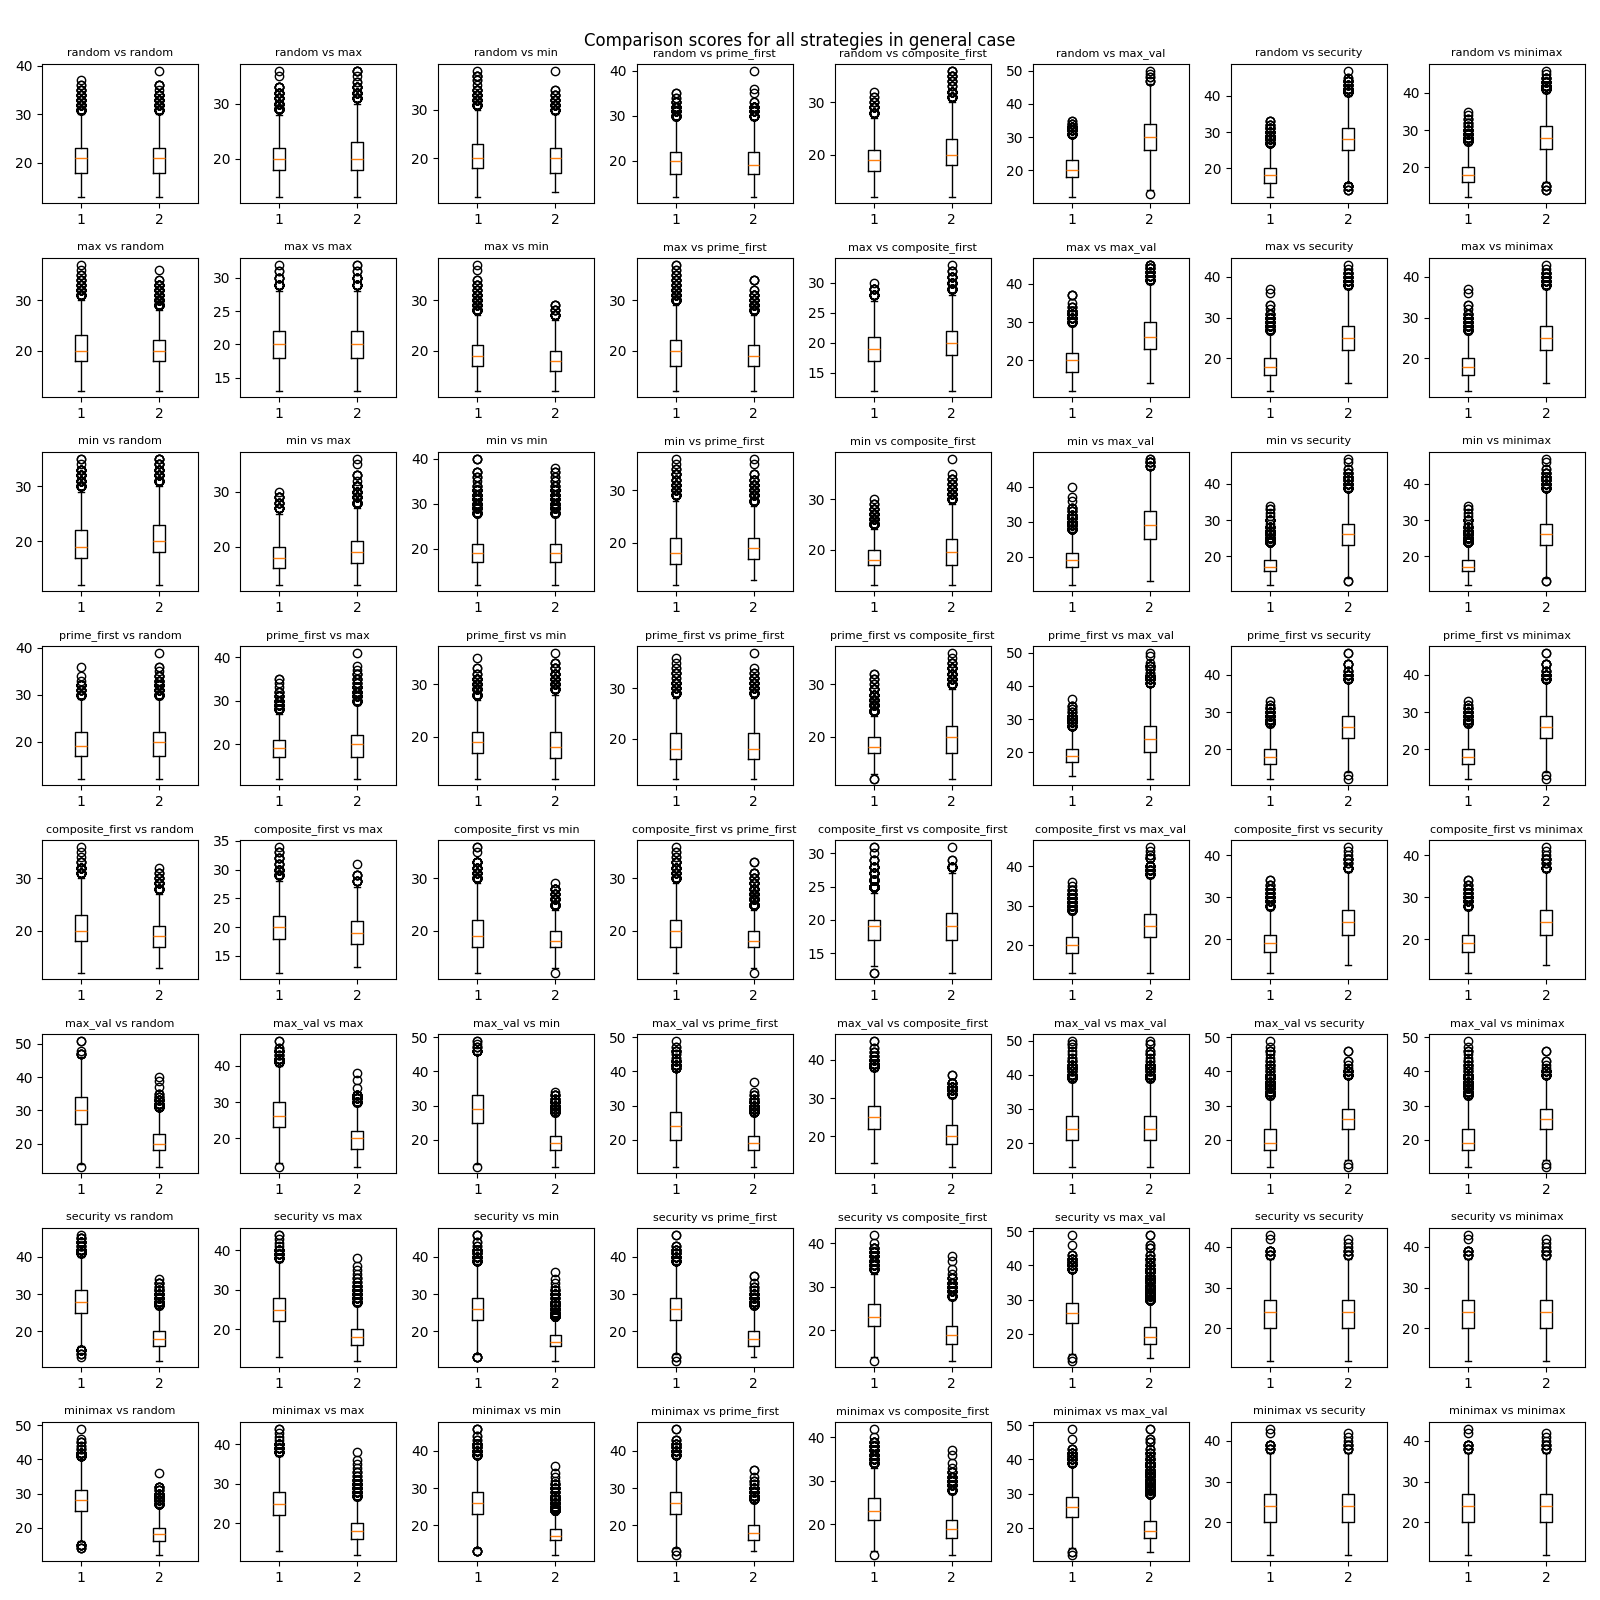
\includegraphics[width=1\linewidth]{img/scores_general.png}
	\caption{Plot that reports the box plots of the different score for each pair of strategies in the general case.}
	\label{fig:box_general}
\end{figure}

\begin{figure}
	\centering
	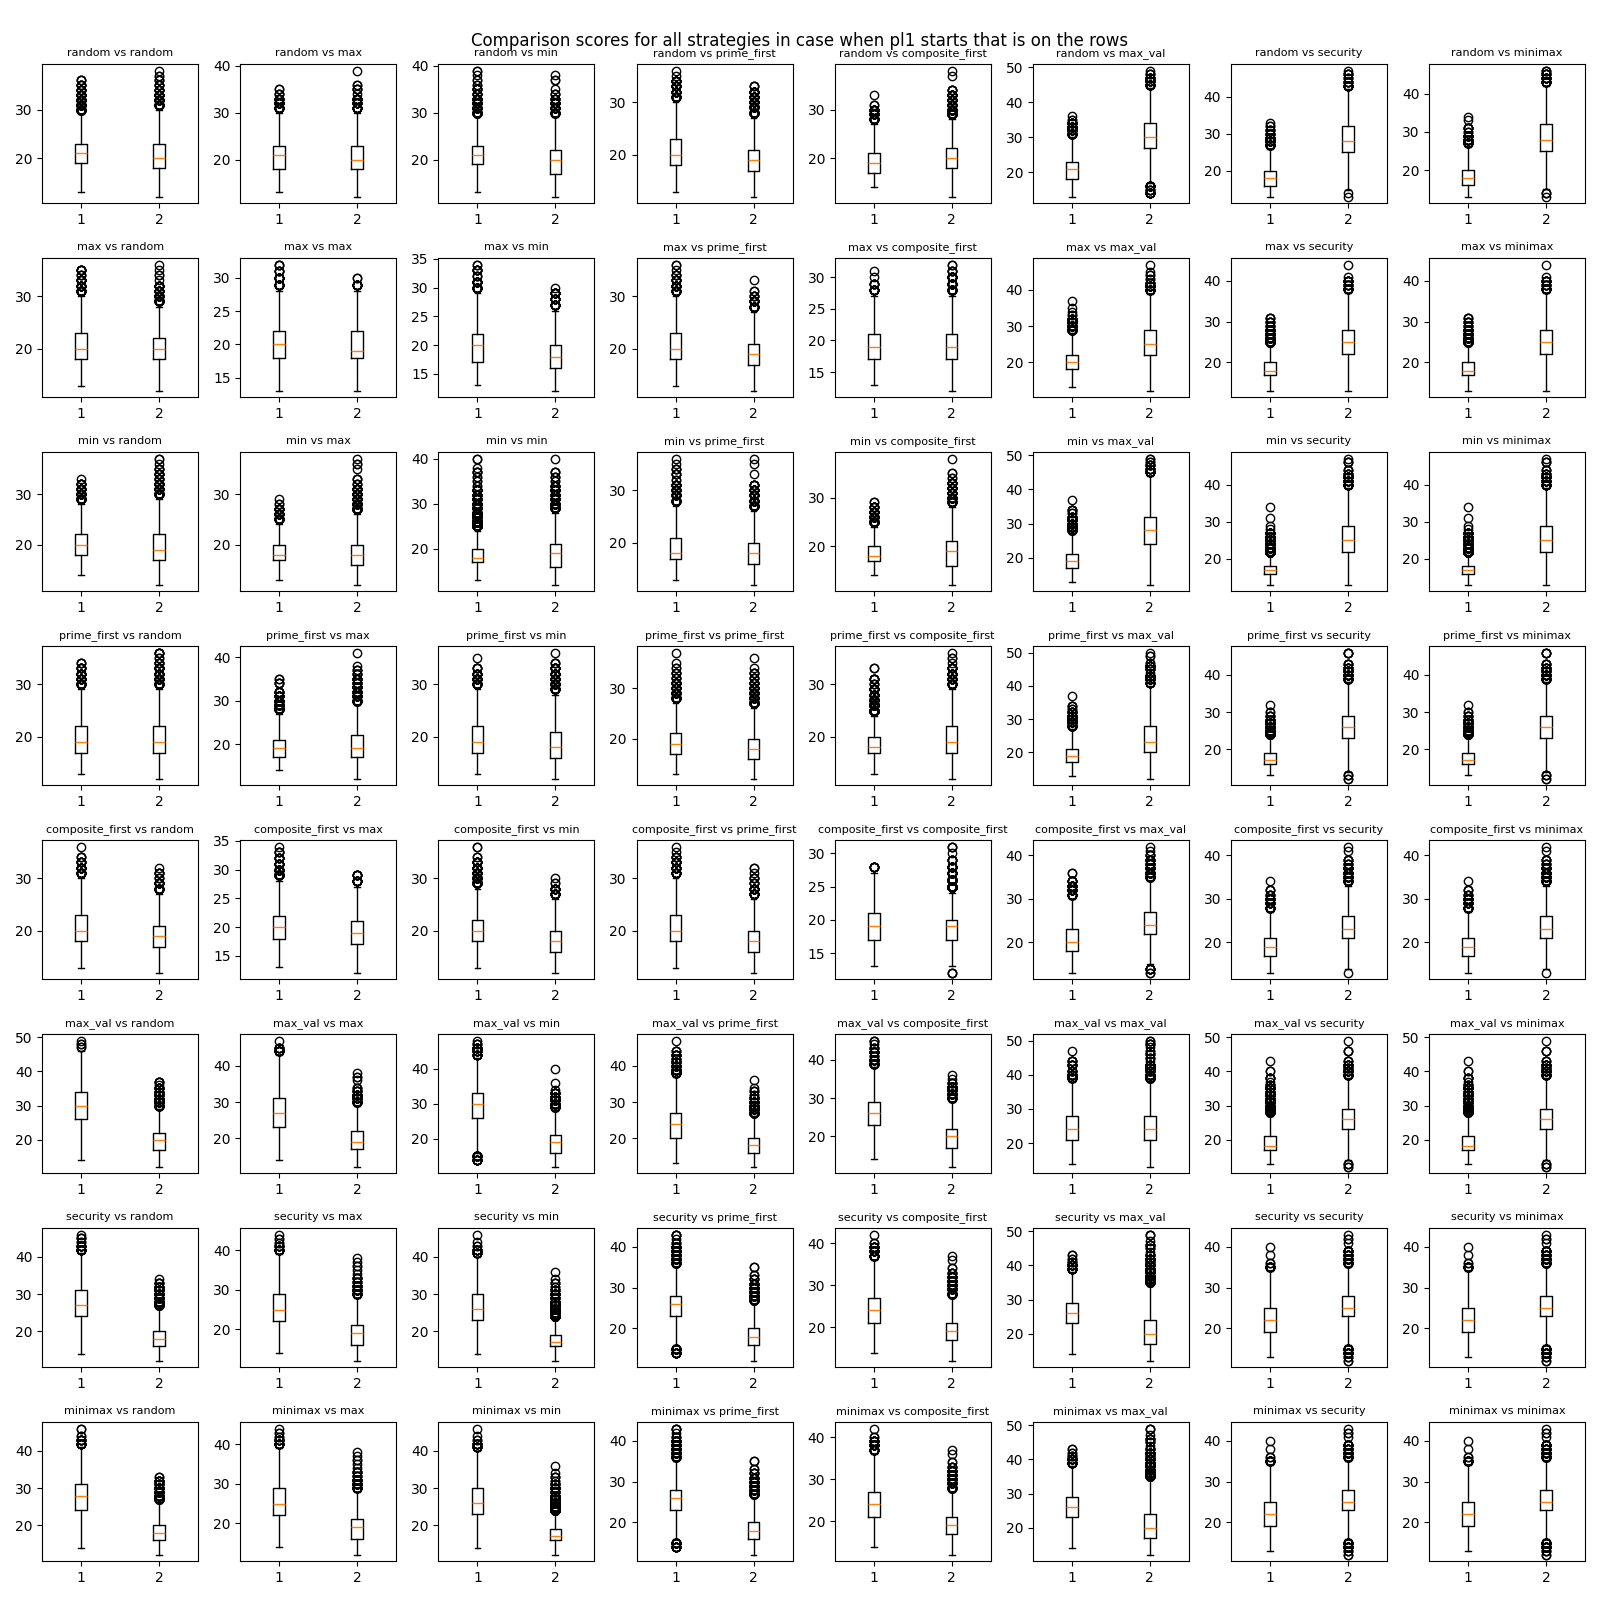
\includegraphics[width=1\linewidth]{img/scores_p1first.png}
	\caption{Plot that reports the box plots of the different score for each pair of strategies when player 1 starts.}
	\label{fig:box_starts}
\end{figure}

In order to better visualize the distribution of the box plots, we restricted the strategies to random, max\_val, security and minimax, since they are the most significant. The results can bee seen in Figures \ref{fig:box_general_rel} and \ref{fig:box_starts_rel}.

\textbf{WRONG PLOTS}

\begin{figure}
	\centering
	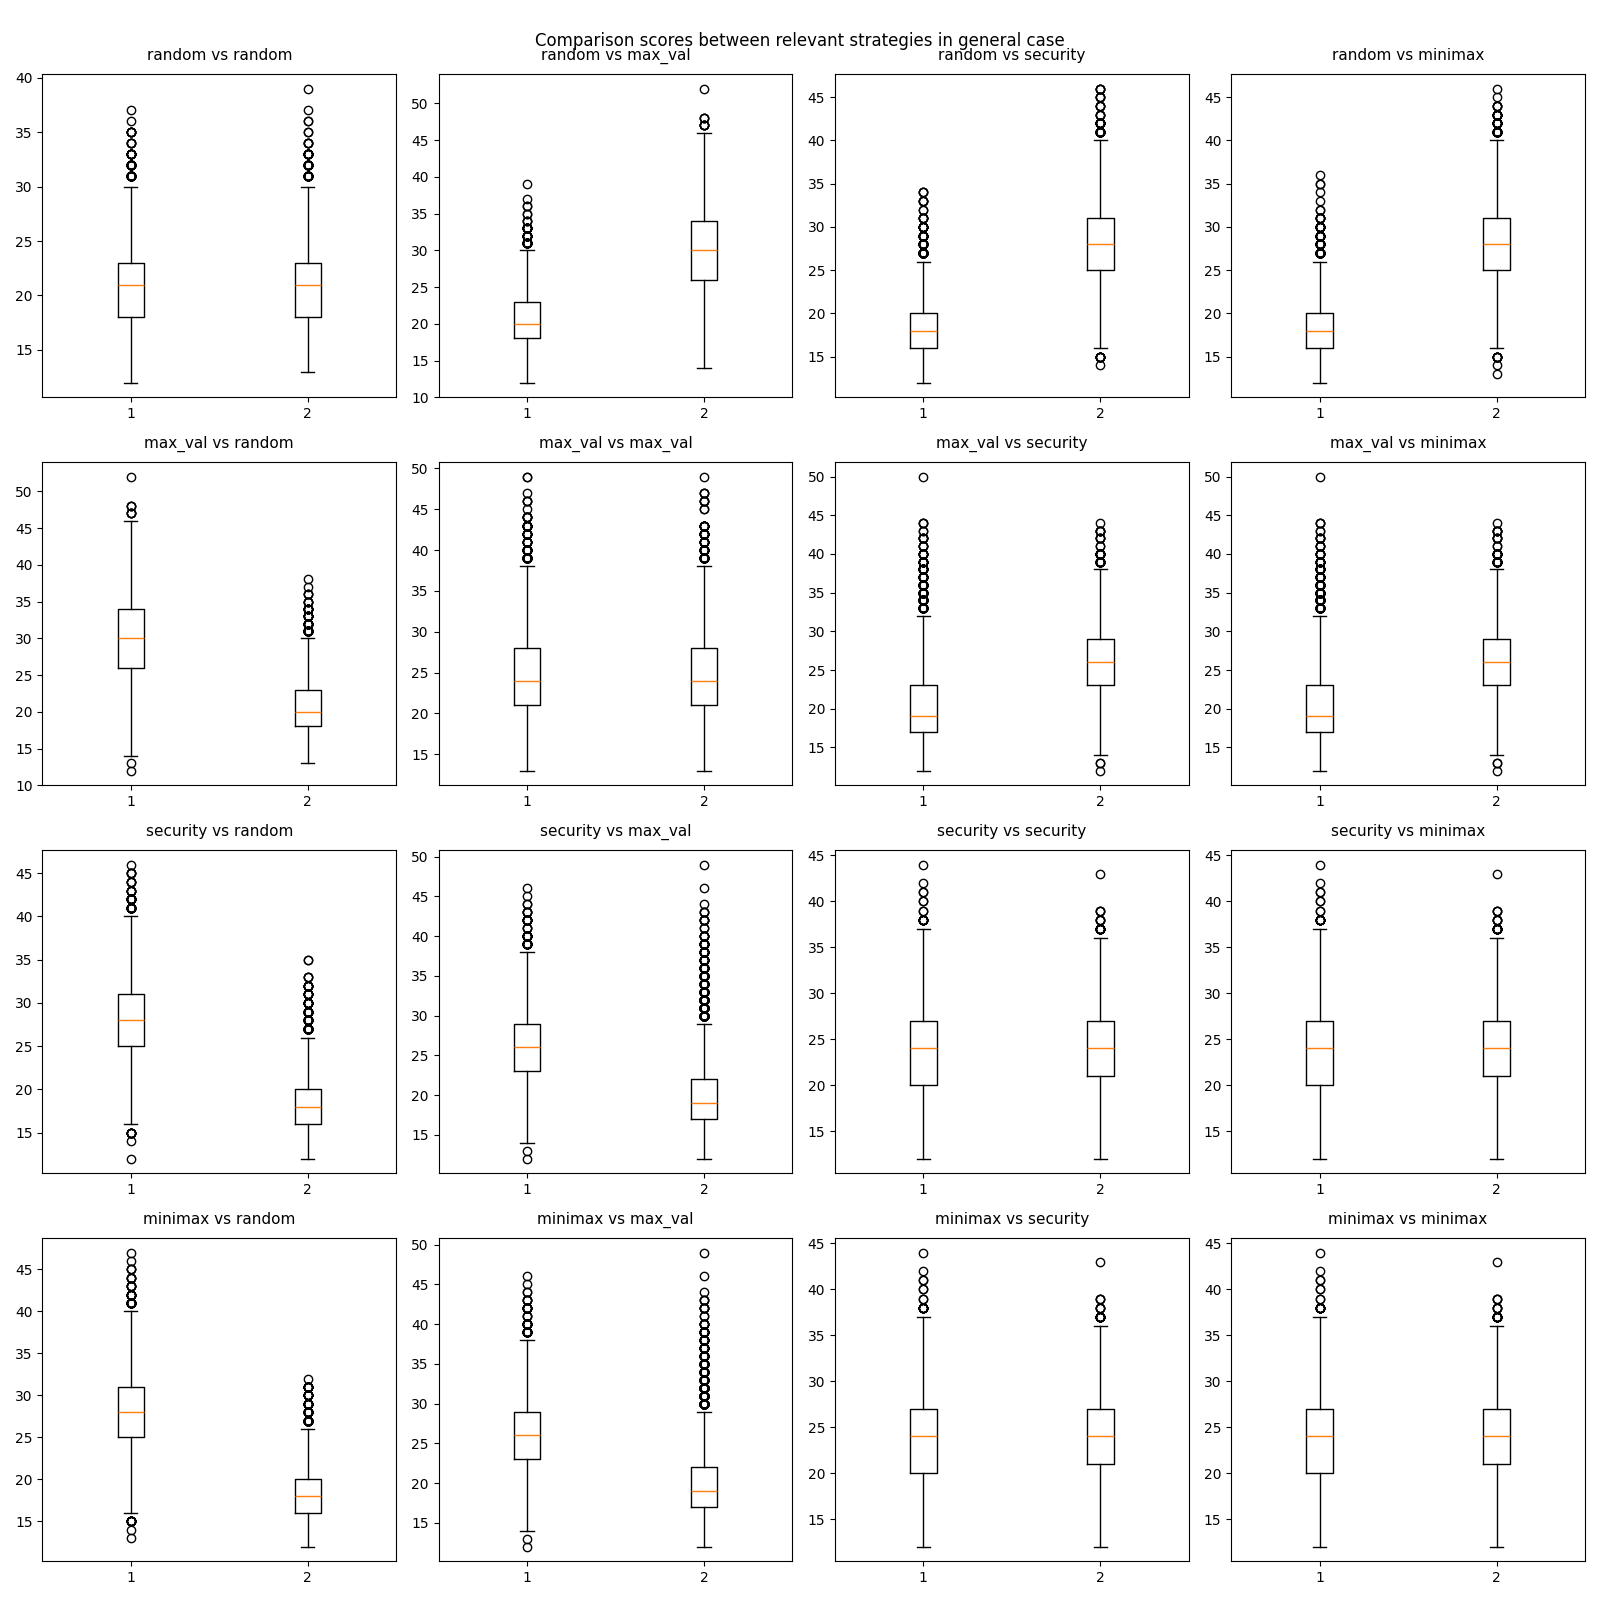
\includegraphics[width=1\linewidth]{img/scores_general_rel.png}
	\caption{Plot that reports the box plots of the different score for each pair of strategies in the general case.}
	\label{fig:box_general_rel}
\end{figure}

\begin{figure}
	\centering
	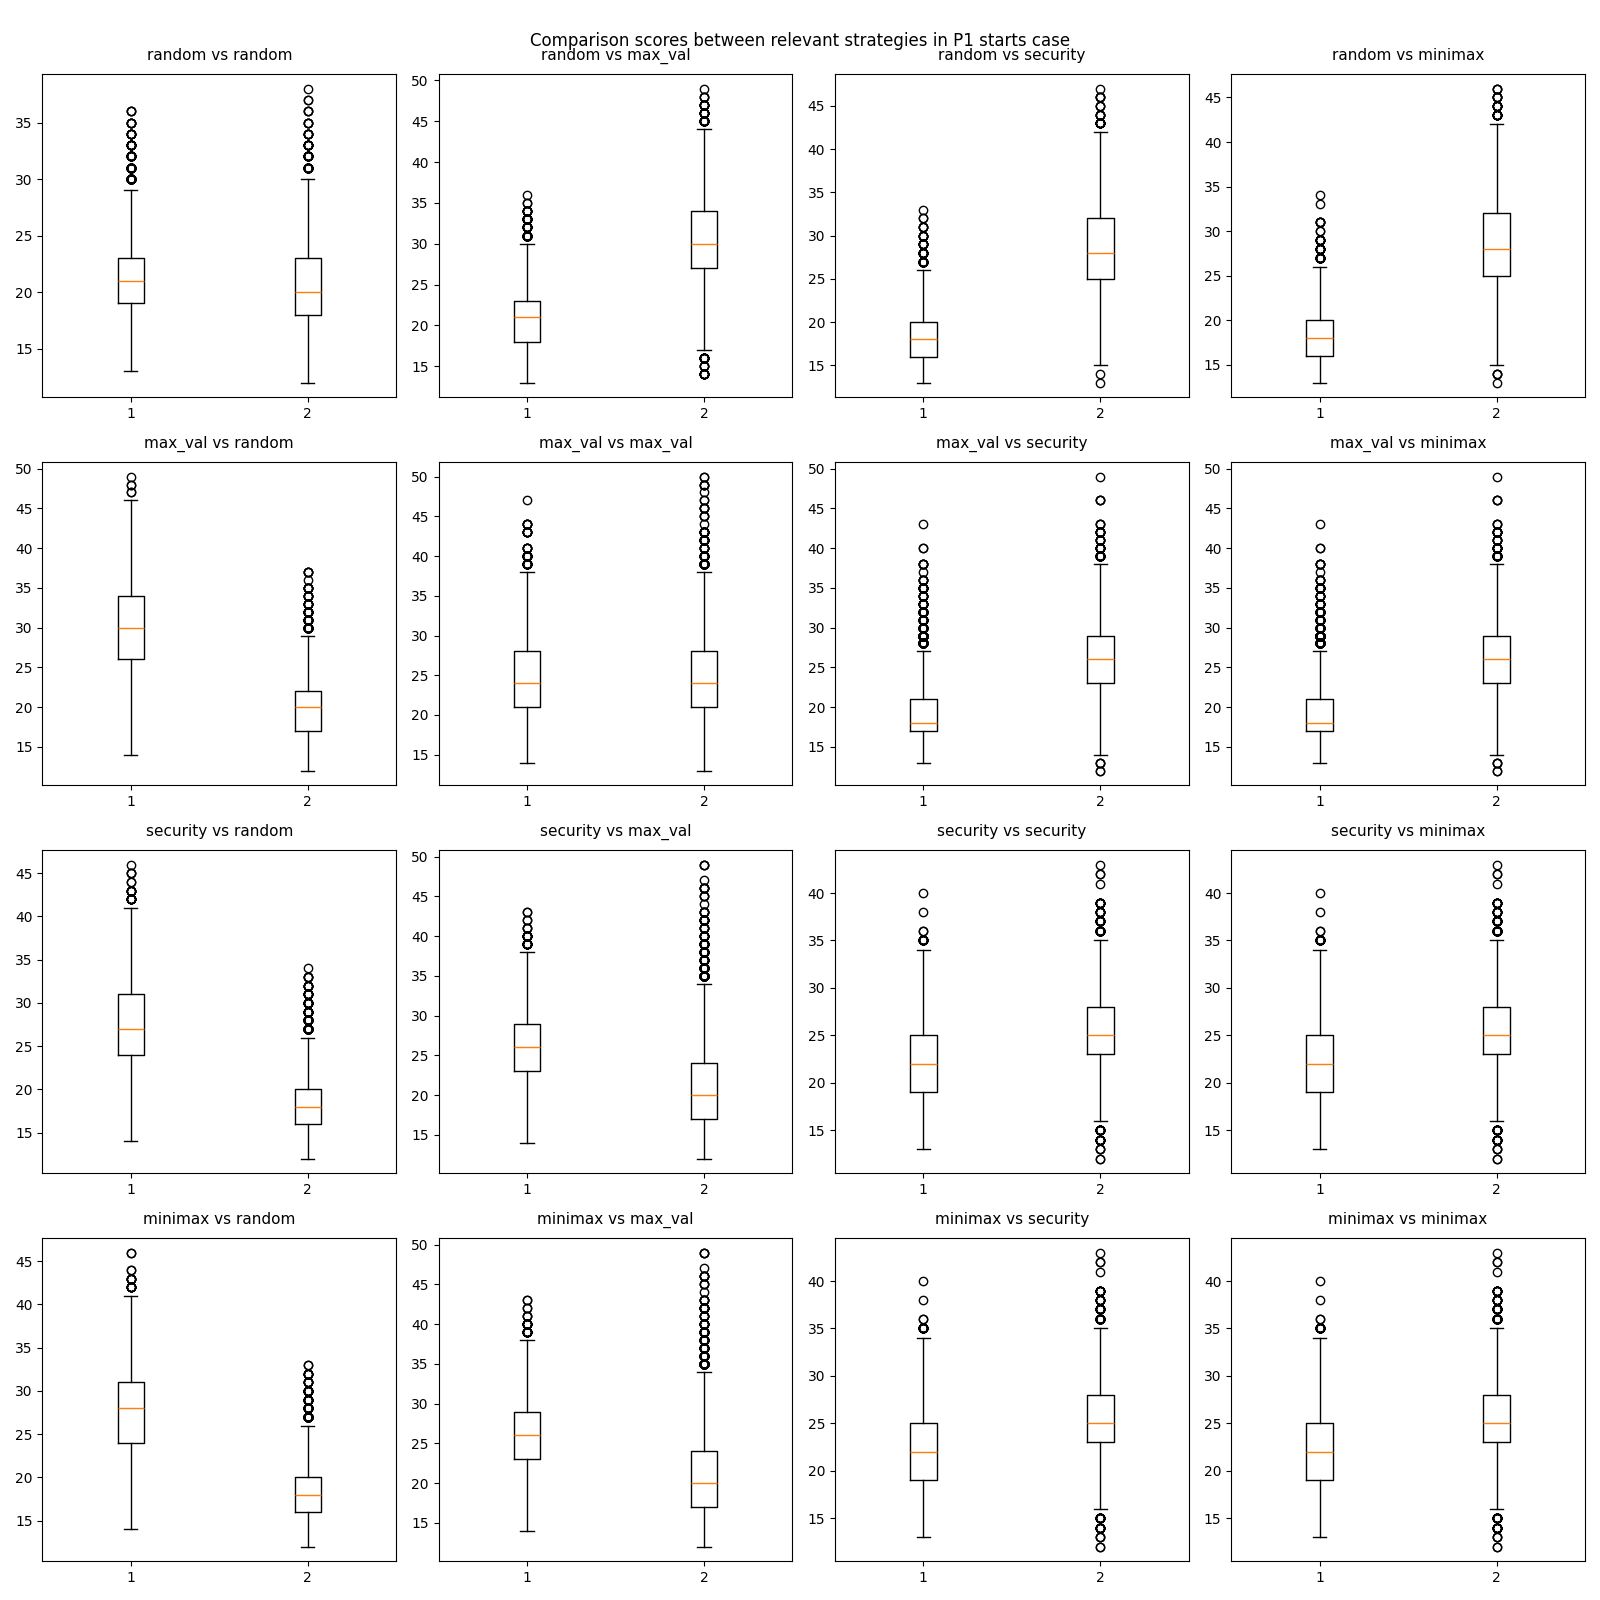
\includegraphics[width=1\linewidth]{img/scores_p1first_rel.png}
	\caption{Plot that reports the box plots of the different score for each pair of strategies when player 1 starts.}
	\label{fig:box_starts_rel}
\end{figure}

From the comparison between those restricted plots, we can see again reflected many of the results discussed in Section \ref{}.
We can see again the bottom left part where we have a worsening of the scores of player 1 from general to the case where it starts confirming again what we have said before. 
Also, we can see that, in general, we have very small boxes but very large whiskers; this means that we have a large variance of the scores but also that in the 2\textsuperscript{nd} and 3\textsuperscript{rd} quantiles we have data that is very concentrated. We can also see that there are a lot of outliers pretty much everywhere. In particular, we can see that when player 1 starts, the number of outliers increases a lot for both players.

At the end of the code, there is also a small part that uses an optimization method to find the binomial distribution that best fits the data in the two cases. The distributions found are very similar to the ones computed before using the equation \ref{eq:probability_cal}.